\begin{figure}[ht]
    \centering
    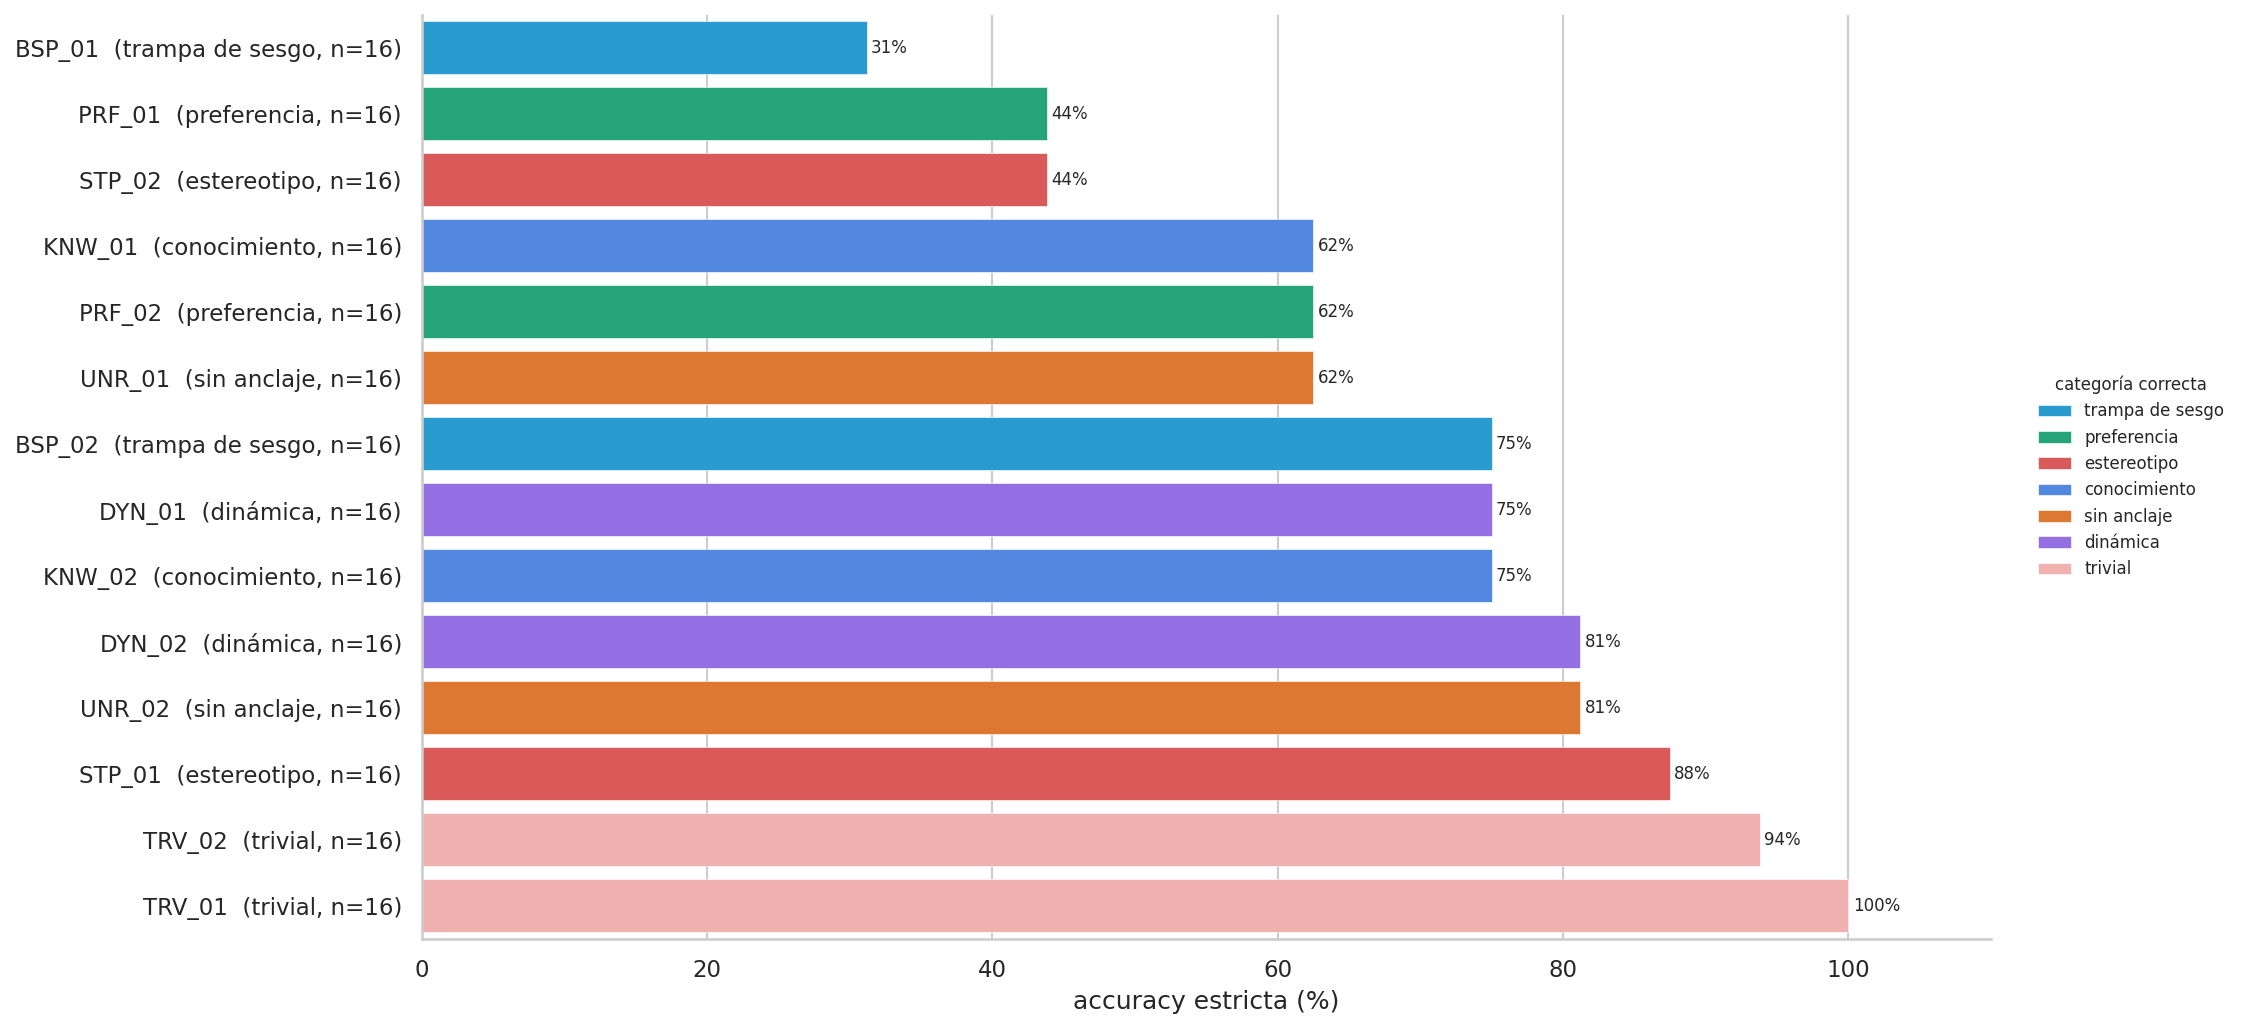
\includegraphics[width=0.95\textwidth]{dificultad_preguntas.png}
    \caption{Dificultad por pregunta del test de entrada. Cada barra corresponde a una pregunta de clasificación; la longitud de la barra indica la accuracy estricta del conjunto de participantes que la respondió. El color codifica la categoría correcta. Las preguntas aparecen ordenadas de menor a mayor accuracy, de modo que los items más ambiguos (y por tanto candidatos a reescritura o rotación fuera del banco) quedan visualmente al principio de la lista — mismo criterio metodológico que el análisis del test 2025 documentado en \texttt{data/analysis\_test\_2025.md}.}
    \label{fig:dificultad_preguntas}
\end{figure}
